\documentclass{standalone}
\usepackage{tikz}
\usetikzlibrary{positioning, topaths}

\begin{document}
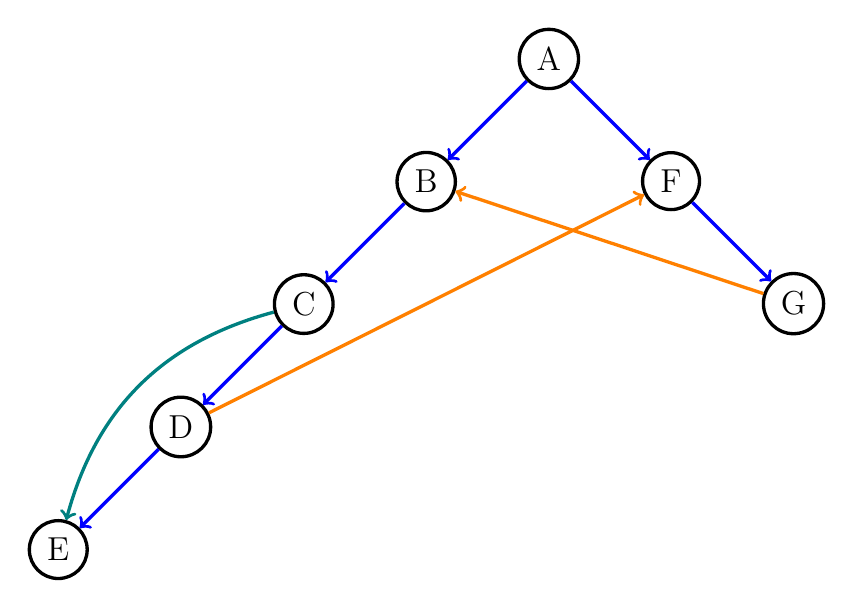
\begin{tikzpicture}[every node/.style = {draw, very thick, circle, font = \large, minimum size = 3pt}, 
  cross/.style = {very thick, orange}, back/.style = {very thick, teal}, tree/.style = {very thick, blue}]
  \node (a) {A};
  \node[below left = of a] (b) {B};
  \node[below left = of b] (c) {C};
  \node[below left = of c] (d) {D};
  \node[below left = of d] (e) {E};
  
  \path[->] (a) edge[tree] (b)
	(b) edge[tree] (c)
	(c) edge[tree] (d)
	(d) edge[tree] (e);

  \node[below right = of a] (f) {F};
  \node[below right = of f] (g) {G};
  \path[->] (a) edge[tree] (f) 
	(f) edge[tree] (g);

  \path[->] (g) edge[cross] (b);
  \path[->] (d) edge[cross] (f);
  \path[->] (c) edge[back, bend right] (e);
\end{tikzpicture}
\end{document}
